\documentclass[a4paper,11pt]{article}
\usepackage{amsmath,amsthm,amsfonts,amssymb,amscd,amstext,vmargin,graphics,graphicx,tabularx,multicol} \usepackage[french]{babel}
\usepackage[utf8]{inputenc}  
\usepackage[T1]{fontenc} 
\usepackage[T1]{fontenc}
\usepackage{amsmath,amssymb}
\usepackage{pstricks-add,tikz,tkz-tab,variations}
\usepackage[autolanguage,np]{numprint} 

\setmarginsrb{1.5cm}{0.5cm}{1cm}{0.5cm}{0cm}{0cm}{0cm}{0cm} %Gauche, haut, droite, haut
\newcounter{numexo}
\newcommand{\exo}[1]{\stepcounter{numexo}\noindent{\bf Exercice~\thenumexo} : \marginpar{\hfill /#1}}
\reversemarginpar


\newcounter{enumtabi}
\newcounter{enumtaba}
\newcommand{\q}{\stepcounter{enumtabi} \theenumtabi.  }
\newcommand{\qa}{\stepcounter{enumtaba} (\alph{enumtaba}) }
\newcommand{\initq}{\setcounter{enumtabi}{0}}
\newcommand{\initqa}{\setcounter{enumtaba}{0}}

\newcommand{\be}{\begin{enumerate}}
\newcommand{\ee}{\end{enumerate}}
\newcommand{\bi}{\begin{itemize}}
\newcommand{\ei}{\end{itemize}}
\newcommand{\bp}{\begin{pspicture*}}
\newcommand{\ep}{\end{pspicture*}}
\newcommand{\bt}{\begin{tabular}}
\newcommand{\et}{\end{tabular}}
\renewcommand{\tabularxcolumn}[1]{>{\centering}m{#1}} %(colonne m{} centrée, au lieu de p par défault) 
\newcommand{\tnl}{\tabularnewline}

\newcommand{\trait}{\noindent \rule{\linewidth}{0.2mm}}
\newcommand{\hs}[1]{\hspace{#1}}
\newcommand{\vs}[1]{\vspace{#1}}

\newcommand{\N}{\mathbb{N}}
\newcommand{\Z}{\mathbb{Z}}
\newcommand{\R}{\mathbb{R}}
\newcommand{\C}{\mathbb{C}}
\newcommand{\Dcal}{\mathcal{D}}
\newcommand{\Ccal}{\mathcal{C}}
\newcommand{\mc}{\mathcal}

\newcommand{\vect}[1]{\overrightarrow{#1}}
\newcommand{\ds}{\displaystyle}
\newcommand{\eq}{\quad \Leftrightarrow \quad}
\newcommand{\vecti}{\vec{\imath}}
\newcommand{\vectj}{\vec{\jmath}}
\newcommand{\Oij}{(O;\vec{\imath}, \vec{\jmath})}
\newcommand{\OIJ}{(O;I,J)}

\newcommand{\bmul}[1]{\begin{multicols}{#1}}
\newcommand{\emul}{\end{multicols}}


\newcommand{\reponse}[1][1]{%
\multido{}{#1}{\makebox[\linewidth]{\rule[0pt]{0pt}{20pt}\dotfill}
}}

\newcommand{\titre}[5] 
% #1: titre #2: haut gauche #3: bas gauche #4: haut droite #5: bas droite
{
\noindent #2 \hfill #4 \\
#3 \hfill #5

\vspace{-1.6cm}

\begin{center}\rule{6cm}{0.5mm}\end{center}
\vspace{0.2cm}
\begin{center}{\large{\textbf{#1}}}\end{center}
\begin{center}\rule{6cm}{0.5mm}\end{center}
}



\begin{document}
\pagestyle{empty}
\titre{Interrogation : Parallélogrammes }{Nom :}{Prénom :}{Classe}{Date}


\exo{3}  Cours\\

\q Donner la définition d'un parallélogramme.\\
\reponse[2]\\

\q Tracer le quadrilatère KLMN pour que KLMN soit un parallélogramme de centre O :

\begin{center}
\includegraphics[scale=1]{para.eps} 
\end{center}

\bmul{2}
\q Nommer quatre parallélogrammes dans la figure ci-contre, 
en sachant que :  (AH)$\slash\slash$(CJ) ; (BG) $\slash\slash$(DI) ; (AD)$\slash\slash$(EF)$\slash\slash$(GJ)  :

\columnbreak

\includegraphics[scale=1]{fig1.eps} 

\emul
\noindent \reponse[2]\\



\exo{3} 

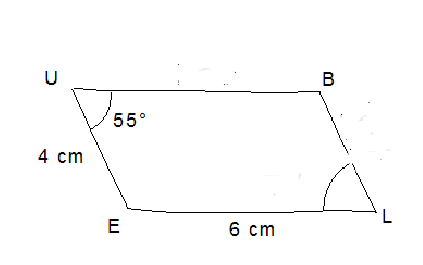
\includegraphics[scale=1]{demo1.eps} 

\initq
\q Le quadrilatère BLEU est un parallélogramme. Quel est la mesure de l'angle $\widehat{BLE}$ ? (Une démonstration est attendue)

\noindent \reponse[4]


\includegraphics[scale=1]{demo2.eps} 

\q Quel est la mesure de la longueur IO? (Une démonstration est attendue)

\noindent \reponse[4]



\exo{2} 

\initq \q Démontrer que le quadrilatère ci-dessous est un parallélogramme.

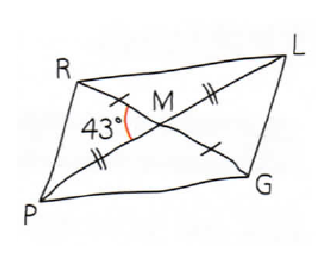
\includegraphics[scale=1]{fig2.eps} 

\noindent\reponse[5]\\
										
\q Quel est la mesure de l'angle $\widehat{LMG}$ ?\\
\reponse[2]\\




\exo{2} Dire si l'affirmation est vraie ou fausse 	\\

\qa Tout parallélogramme a un axe de symétrie : .....................\\

\qa Un parallélogramme peut avoir un angle de 28 degré et un angle de 62 degré : ...................\\

\qa Si LYNX est un parallélogramme, alors LX = YN : ...................\\

\qa Si CHAT est un parallélogramme de centre O, alors les triangles COH et AOT ont le même périmètre :.......................\\





\end{document}
